\documentclass[twoside]{book}

% Packages required by doxygen
\usepackage{fixltx2e}
\usepackage{calc}
\usepackage{doxygen}
\usepackage[export]{adjustbox} % also loads graphicx
\usepackage{graphicx}
\usepackage[utf8]{inputenc}
\usepackage{makeidx}
\usepackage{multicol}
\usepackage{multirow}
\PassOptionsToPackage{warn}{textcomp}
\usepackage{textcomp}
\usepackage[nointegrals]{wasysym}
\usepackage[table]{xcolor}

% Font selection
\usepackage[T1]{fontenc}
\usepackage[scaled=.90]{helvet}
\usepackage{courier}
\usepackage{amssymb}
\usepackage{sectsty}
\renewcommand{\familydefault}{\sfdefault}
\allsectionsfont{%
  \fontseries{bc}\selectfont%
  \color{darkgray}%
}
\renewcommand{\DoxyLabelFont}{%
  \fontseries{bc}\selectfont%
  \color{darkgray}%
}
\newcommand{\+}{\discretionary{\mbox{\scriptsize$\hookleftarrow$}}{}{}}

% Page & text layout
\usepackage{geometry}
\geometry{%
  a4paper,%
  top=2.5cm,%
  bottom=2.5cm,%
  left=2.5cm,%
  right=2.5cm%
}
\tolerance=750
\hfuzz=15pt
\hbadness=750
\setlength{\emergencystretch}{15pt}
\setlength{\parindent}{0cm}
\setlength{\parskip}{3ex plus 2ex minus 2ex}
\makeatletter
\renewcommand{\paragraph}{%
  \@startsection{paragraph}{4}{0ex}{-1.0ex}{1.0ex}{%
    \normalfont\normalsize\bfseries\SS@parafont%
  }%
}
\renewcommand{\subparagraph}{%
  \@startsection{subparagraph}{5}{0ex}{-1.0ex}{1.0ex}{%
    \normalfont\normalsize\bfseries\SS@subparafont%
  }%
}
\makeatother

% Headers & footers
\usepackage{fancyhdr}
\pagestyle{fancyplain}
\fancyhead[LE]{\fancyplain{}{\bfseries\thepage}}
\fancyhead[CE]{\fancyplain{}{}}
\fancyhead[RE]{\fancyplain{}{\bfseries\leftmark}}
\fancyhead[LO]{\fancyplain{}{\bfseries\rightmark}}
\fancyhead[CO]{\fancyplain{}{}}
\fancyhead[RO]{\fancyplain{}{\bfseries\thepage}}
\fancyfoot[LE]{\fancyplain{}{}}
\fancyfoot[CE]{\fancyplain{}{}}
\fancyfoot[RE]{\fancyplain{}{\bfseries\scriptsize Generated by Doxygen }}
\fancyfoot[LO]{\fancyplain{}{\bfseries\scriptsize Generated by Doxygen }}
\fancyfoot[CO]{\fancyplain{}{}}
\fancyfoot[RO]{\fancyplain{}{}}
\renewcommand{\footrulewidth}{0.4pt}
\renewcommand{\chaptermark}[1]{%
  \markboth{#1}{}%
}
\renewcommand{\sectionmark}[1]{%
  \markright{\thesection\ #1}%
}

% Indices & bibliography
\usepackage{natbib}
\usepackage[titles]{tocloft}
\setcounter{tocdepth}{3}
\setcounter{secnumdepth}{5}
\makeindex

% Hyperlinks (required, but should be loaded last)
\usepackage{ifpdf}
\ifpdf
  \usepackage[pdftex,pagebackref=true]{hyperref}
\else
  \usepackage[ps2pdf,pagebackref=true]{hyperref}
\fi
\hypersetup{%
  colorlinks=true,%
  linkcolor=blue,%
  citecolor=blue,%
  unicode%
}

% Custom commands
\newcommand{\clearemptydoublepage}{%
  \newpage{\pagestyle{empty}\cleardoublepage}%
}

\usepackage{caption}
\captionsetup{labelsep=space,justification=centering,font={bf},singlelinecheck=off,skip=4pt,position=top}

%===== C O N T E N T S =====

\begin{document}

% Titlepage & ToC
\hypersetup{pageanchor=false,
             bookmarksnumbered=true,
             pdfencoding=unicode
            }
\pagenumbering{alph}
\begin{titlepage}
\vspace*{7cm}
\begin{center}%
{\Large Strategy }\\
\vspace*{1cm}
{\large Generated by Doxygen 1.8.13}\\
\end{center}
\end{titlepage}
\clearemptydoublepage
\pagenumbering{roman}
\tableofcontents
\clearemptydoublepage
\pagenumbering{arabic}
\hypersetup{pageanchor=true}

%--- Begin generated contents ---
\chapter{Namespace Index}
\section{Packages}
Here are the packages with brief descriptions (if available)\+:\begin{DoxyCompactList}
\item\contentsline{section}{\hyperlink{namespace_decorator}{Decorator} }{\pageref{namespace_decorator}}{}
\end{DoxyCompactList}

\chapter{Hierarchical Index}
\section{Class Hierarchy}
This inheritance list is sorted roughly, but not completely, alphabetically\+:\begin{DoxyCompactList}
\item \contentsline{section}{Strategy.\+Dojazd}{\pageref{interface_strategy_1_1_dojazd}}{}
\begin{DoxyCompactList}
\item \contentsline{section}{Strategy.\+Rower}{\pageref{class_strategy_1_1_rower}}{}
\item \contentsline{section}{Strategy.\+Samochod}{\pageref{class_strategy_1_1_samochod}}{}
\end{DoxyCompactList}
\item \contentsline{section}{Strategy.\+Praca}{\pageref{interface_strategy_1_1_praca}}{}
\begin{DoxyCompactList}
\item \contentsline{section}{Strategy.\+Maluje\+Samochod}{\pageref{class_strategy_1_1_maluje_samochod}}{}
\item \contentsline{section}{Strategy.\+Montuje\+Silnik}{\pageref{class_strategy_1_1_montuje_silnik}}{}
\item \contentsline{section}{Strategy.\+Testuje\+Samochodow}{\pageref{class_strategy_1_1_testuje_samochodow}}{}
\end{DoxyCompactList}
\item \contentsline{section}{Strategy.\+Pracownik}{\pageref{class_strategy_1_1_pracownik}}{}
\item \contentsline{section}{Strategy.\+Spedzanie\+Wolnego\+Czasu}{\pageref{interface_strategy_1_1_spedzanie_wolnego_czasu}}{}
\begin{DoxyCompactList}
\item \contentsline{section}{Strategy.\+Gra\+Komputerowa}{\pageref{class_strategy_1_1_gra_komputerowa}}{}
\item \contentsline{section}{Strategy.\+Literatura\+Popularno\+Naukowa}{\pageref{class_strategy_1_1_literatura_popularno_naukowa}}{}
\item \contentsline{section}{Strategy.\+Silownia}{\pageref{class_strategy_1_1_silownia}}{}
\end{DoxyCompactList}
\item \contentsline{section}{Strategy.\+Strategy}{\pageref{class_strategy_1_1_strategy}}{}
\end{DoxyCompactList}

\chapter{Class Index}
\section{Class List}
Here are the classes, structs, unions and interfaces with brief descriptions\+:\begin{DoxyCompactList}
\item\contentsline{section}{\hyperlink{class_lazy_1_1_custom_lazy_class}{Lazy.\+Custom\+Lazy\+Class} \\*\hyperlink{class_lazy_1_1_custom_lazy_class}{Custom\+Lazy\+Class} posiada zmienna \+\_\+\+Value inicjalizowaną tuż przed uzyciem }{\pageref{class_lazy_1_1_custom_lazy_class}}{}
\item\contentsline{section}{\hyperlink{class_lazy_1_1_lazy}{Lazy.\+Lazy} \\*Klasa zawierająca funkcje Main }{\pageref{class_lazy_1_1_lazy}}{}
\item\contentsline{section}{\hyperlink{class_lazy_1_1_lazy_class}{Lazy.\+Lazy\+Class} \\*\hyperlink{class_lazy_1_1_lazy_class}{Lazy\+Class} posiada zmienna Value }{\pageref{class_lazy_1_1_lazy_class}}{}
\end{DoxyCompactList}

\chapter{Namespace Documentation}
\hypertarget{namespace_strategy}{}\section{Strategy Namespace Reference}
\label{namespace_strategy}\index{Strategy@{Strategy}}
\subsection*{Classes}
\begin{DoxyCompactItemize}
\item 
interface \hyperlink{interface_strategy_1_1_dojazd}{Dojazd}
\begin{DoxyCompactList}\small\item\em Interface wymagający implementacji funkcji dojazd \end{DoxyCompactList}\item 
class \hyperlink{class_strategy_1_1_gra_komputerowa}{Gra\+Komputerowa}
\begin{DoxyCompactList}\small\item\em Klasa implementacji funkcje spedzaj\+Wolny\+Czas \end{DoxyCompactList}\item 
class \hyperlink{class_strategy_1_1_literatura_popularno_naukowa}{Literatura\+Popularno\+Naukowa}
\begin{DoxyCompactList}\small\item\em Klasa implementacji funkcje spedzaj\+Wolny\+Czas \end{DoxyCompactList}\item 
class \hyperlink{class_strategy_1_1_maluje_samochod}{Maluje\+Samochod}
\begin{DoxyCompactList}\small\item\em Klasa implementacji funkcje pracuj \end{DoxyCompactList}\item 
class \hyperlink{class_strategy_1_1_montuje_silnik}{Montuje\+Silnik}
\begin{DoxyCompactList}\small\item\em Klasa implementacji funkcje pracuj \end{DoxyCompactList}\item 
interface \hyperlink{interface_strategy_1_1_praca}{Praca}
\begin{DoxyCompactList}\small\item\em Interface wymagający implementacji funkcji pracuj \end{DoxyCompactList}\item 
class \hyperlink{class_strategy_1_1_pracownik}{Pracownik}
\begin{DoxyCompactList}\small\item\em Klasa ustalająca kontekst \end{DoxyCompactList}\item 
class \hyperlink{class_strategy_1_1_rower}{Rower}
\begin{DoxyCompactList}\small\item\em Klasa implementacji funkcje dojazd \end{DoxyCompactList}\item 
class \hyperlink{class_strategy_1_1_samochod}{Samochod}
\begin{DoxyCompactList}\small\item\em Klasa implementacji funkcje dojazd \end{DoxyCompactList}\item 
class \hyperlink{class_strategy_1_1_silownia}{Silownia}
\begin{DoxyCompactList}\small\item\em Klasa implementacji funkcje spedzaj\+Wolny\+Czas \end{DoxyCompactList}\item 
interface \hyperlink{interface_strategy_1_1_spedzanie_wolnego_czasu}{Spedzanie\+Wolnego\+Czasu}
\begin{DoxyCompactList}\small\item\em Interface wymagający implementacji funkcji spedzaj\+Wolny\+Czas \end{DoxyCompactList}\item 
class \hyperlink{class_strategy_1_1_strategy}{Strategy}
\begin{DoxyCompactList}\small\item\em Klasa posiadająca funkcje Main \end{DoxyCompactList}\item 
class \hyperlink{class_strategy_1_1_testuje_samochodow}{Testuje\+Samochodow}
\begin{DoxyCompactList}\small\item\em Klasa implementacji funkcje pracuj \end{DoxyCompactList}\end{DoxyCompactItemize}

\chapter{Class Documentation}
\hypertarget{interface_strategy_1_1_dojazd}{}\section{Strategy.\+Dojazd Interface Reference}
\label{interface_strategy_1_1_dojazd}\index{Strategy.\+Dojazd@{Strategy.\+Dojazd}}


Interface wymagający implementacji funkcji dojazd  


Inheritance diagram for Strategy.\+Dojazd\+:\begin{figure}[H]
\begin{center}
\leavevmode
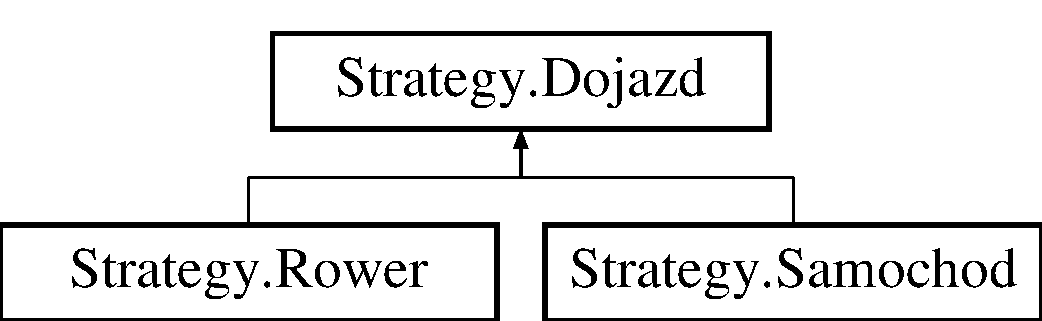
\includegraphics[height=2.000000cm]{interface_strategy_1_1_dojazd}
\end{center}
\end{figure}
\subsection*{Public Member Functions}
\begin{DoxyCompactItemize}
\item 
\mbox{\Hypertarget{interface_strategy_1_1_dojazd_a232e5c090ce441757dbe515a518ffd7f}\label{interface_strategy_1_1_dojazd_a232e5c090ce441757dbe515a518ffd7f}} 
void {\bfseries dojazd} ()
\end{DoxyCompactItemize}


\subsection{Detailed Description}
Interface wymagający implementacji funkcji dojazd 



The documentation for this interface was generated from the following file\+:\begin{DoxyCompactItemize}
\item 
Program.\+cs\end{DoxyCompactItemize}

\hypertarget{class_strategy_1_1_gra_komputerowa}{}\section{Strategy.\+Gra\+Komputerowa Class Reference}
\label{class_strategy_1_1_gra_komputerowa}\index{Strategy.\+Gra\+Komputerowa@{Strategy.\+Gra\+Komputerowa}}


Klasa implementacji funkcje spedzaj\+Wolny\+Czas  


Inheritance diagram for Strategy.\+Gra\+Komputerowa\+:\begin{figure}[H]
\begin{center}
\leavevmode
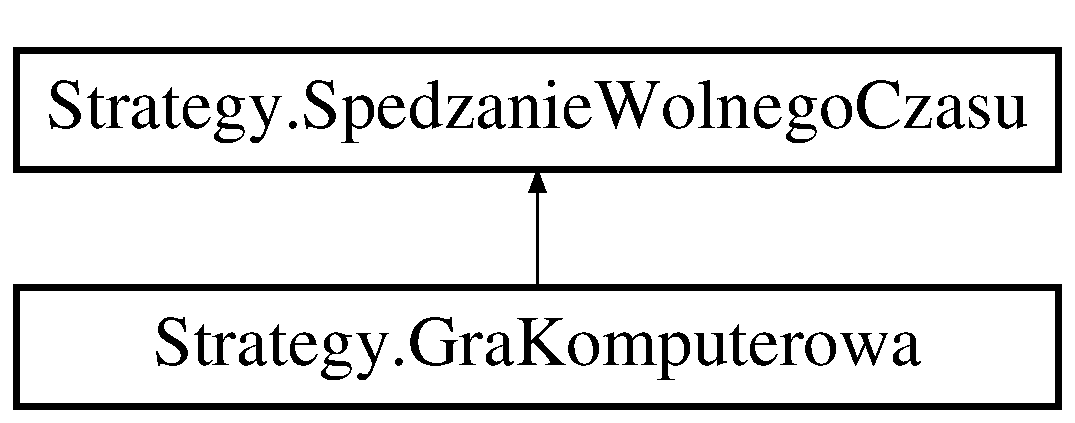
\includegraphics[height=2.000000cm]{class_strategy_1_1_gra_komputerowa}
\end{center}
\end{figure}
\subsection*{Public Member Functions}
\begin{DoxyCompactItemize}
\item 
\mbox{\Hypertarget{class_strategy_1_1_gra_komputerowa_a912ae8e36ee187ff9cf7343751163767}\label{class_strategy_1_1_gra_komputerowa_a912ae8e36ee187ff9cf7343751163767}} 
void {\bfseries spedzaj\+Wolny\+Czas} ()
\end{DoxyCompactItemize}


\subsection{Detailed Description}
Klasa implementacji funkcje spedzaj\+Wolny\+Czas 



The documentation for this class was generated from the following file\+:\begin{DoxyCompactItemize}
\item 
Program.\+cs\end{DoxyCompactItemize}

\hypertarget{class_strategy_1_1_literatura_popularno_naukowa}{}\section{Strategy.\+Literatura\+Popularno\+Naukowa Class Reference}
\label{class_strategy_1_1_literatura_popularno_naukowa}\index{Strategy.\+Literatura\+Popularno\+Naukowa@{Strategy.\+Literatura\+Popularno\+Naukowa}}


Klasa implementacji funkcje spedzaj\+Wolny\+Czas  


Inheritance diagram for Strategy.\+Literatura\+Popularno\+Naukowa\+:\begin{figure}[H]
\begin{center}
\leavevmode
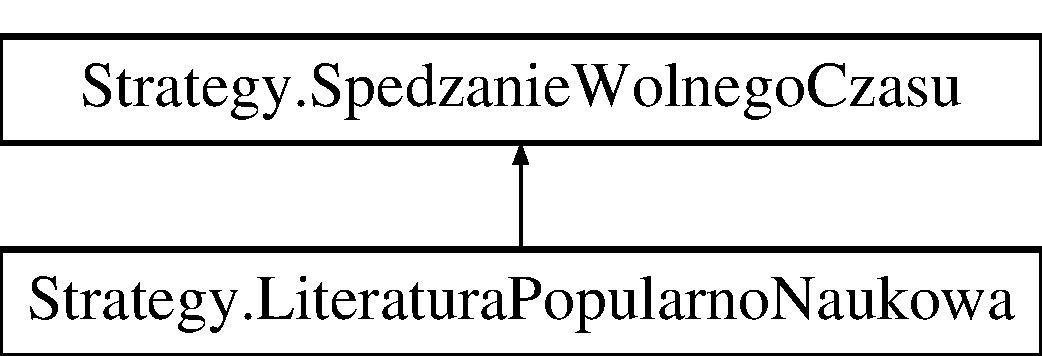
\includegraphics[height=2.000000cm]{class_strategy_1_1_literatura_popularno_naukowa}
\end{center}
\end{figure}
\subsection*{Public Member Functions}
\begin{DoxyCompactItemize}
\item 
\mbox{\Hypertarget{class_strategy_1_1_literatura_popularno_naukowa_a56682dade4c6965a18d3131116cbf495}\label{class_strategy_1_1_literatura_popularno_naukowa_a56682dade4c6965a18d3131116cbf495}} 
void {\bfseries spedzaj\+Wolny\+Czas} ()
\end{DoxyCompactItemize}


\subsection{Detailed Description}
Klasa implementacji funkcje spedzaj\+Wolny\+Czas 



The documentation for this class was generated from the following file\+:\begin{DoxyCompactItemize}
\item 
Program.\+cs\end{DoxyCompactItemize}

\hypertarget{class_strategy_1_1_maluje_samochod}{}\section{Strategy.\+Maluje\+Samochod Class Reference}
\label{class_strategy_1_1_maluje_samochod}\index{Strategy.\+Maluje\+Samochod@{Strategy.\+Maluje\+Samochod}}


Klasa implementacji funkcje pracuj  


Inheritance diagram for Strategy.\+Maluje\+Samochod\+:\begin{figure}[H]
\begin{center}
\leavevmode
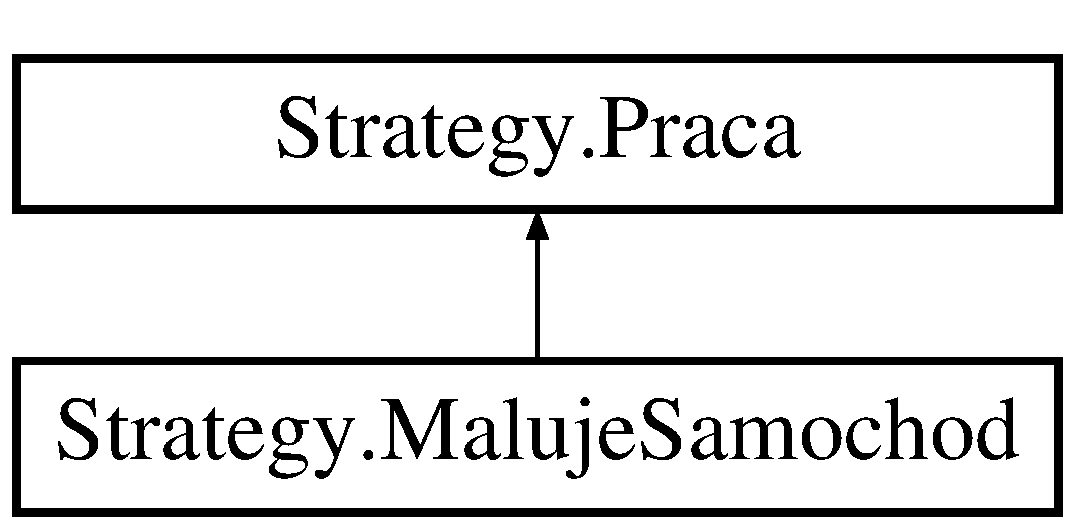
\includegraphics[height=2.000000cm]{class_strategy_1_1_maluje_samochod}
\end{center}
\end{figure}
\subsection*{Public Member Functions}
\begin{DoxyCompactItemize}
\item 
\mbox{\Hypertarget{class_strategy_1_1_maluje_samochod_a9848285874a8eb2da53b5ca69323ffc7}\label{class_strategy_1_1_maluje_samochod_a9848285874a8eb2da53b5ca69323ffc7}} 
void {\bfseries pracuj} ()
\end{DoxyCompactItemize}


\subsection{Detailed Description}
Klasa implementacji funkcje pracuj 



The documentation for this class was generated from the following file\+:\begin{DoxyCompactItemize}
\item 
Program.\+cs\end{DoxyCompactItemize}

\hypertarget{class_strategy_1_1_montuje_silnik}{}\section{Strategy.\+Montuje\+Silnik Class Reference}
\label{class_strategy_1_1_montuje_silnik}\index{Strategy.\+Montuje\+Silnik@{Strategy.\+Montuje\+Silnik}}


Klasa implementacji funkcje pracuj  


Inheritance diagram for Strategy.\+Montuje\+Silnik\+:\begin{figure}[H]
\begin{center}
\leavevmode
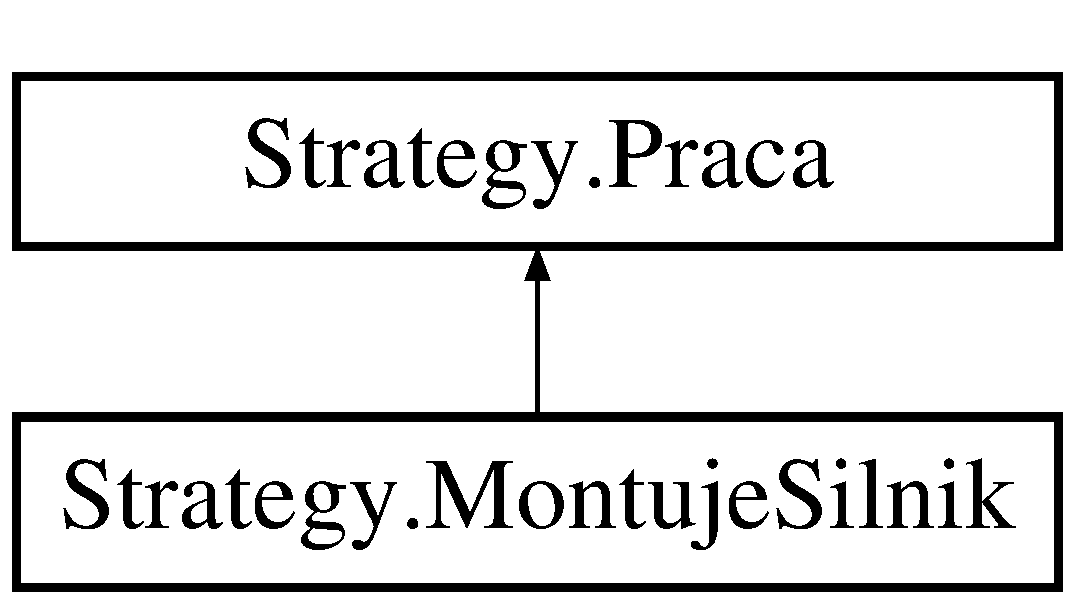
\includegraphics[height=2.000000cm]{class_strategy_1_1_montuje_silnik}
\end{center}
\end{figure}
\subsection*{Public Member Functions}
\begin{DoxyCompactItemize}
\item 
\mbox{\Hypertarget{class_strategy_1_1_montuje_silnik_acf351bbbf344fa57a1d81c9977aa8582}\label{class_strategy_1_1_montuje_silnik_acf351bbbf344fa57a1d81c9977aa8582}} 
void {\bfseries pracuj} ()
\end{DoxyCompactItemize}


\subsection{Detailed Description}
Klasa implementacji funkcje pracuj 



The documentation for this class was generated from the following file\+:\begin{DoxyCompactItemize}
\item 
Program.\+cs\end{DoxyCompactItemize}

\hypertarget{interface_strategy_1_1_praca}{}\section{Strategy.\+Praca Interface Reference}
\label{interface_strategy_1_1_praca}\index{Strategy.\+Praca@{Strategy.\+Praca}}


Interface wymagający implementacji funkcji pracuj  


Inheritance diagram for Strategy.\+Praca\+:\begin{figure}[H]
\begin{center}
\leavevmode
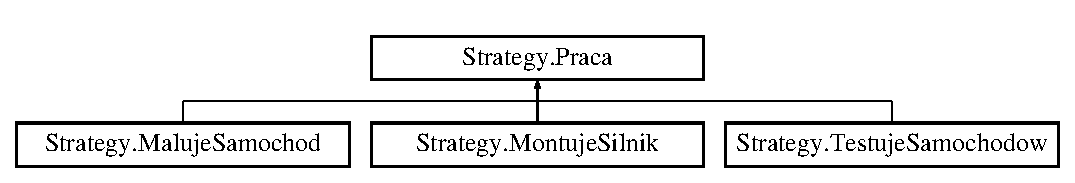
\includegraphics[height=2.000000cm]{interface_strategy_1_1_praca}
\end{center}
\end{figure}
\subsection*{Public Member Functions}
\begin{DoxyCompactItemize}
\item 
\mbox{\Hypertarget{interface_strategy_1_1_praca_a27486a9fd0bbde1361a48bff1855f2b3}\label{interface_strategy_1_1_praca_a27486a9fd0bbde1361a48bff1855f2b3}} 
void {\bfseries pracuj} ()
\end{DoxyCompactItemize}


\subsection{Detailed Description}
Interface wymagający implementacji funkcji pracuj 



The documentation for this interface was generated from the following file\+:\begin{DoxyCompactItemize}
\item 
Program.\+cs\end{DoxyCompactItemize}

\hypertarget{class_strategy_1_1_pracownik}{}\section{Strategy.\+Pracownik Class Reference}
\label{class_strategy_1_1_pracownik}\index{Strategy.\+Pracownik@{Strategy.\+Pracownik}}


Klasa ustalająca kontekst  


\subsection*{Public Member Functions}
\begin{DoxyCompactItemize}
\item 
\mbox{\Hypertarget{class_strategy_1_1_pracownik_a93cd66843cd697fbeadec67a60097017}\label{class_strategy_1_1_pracownik_a93cd66843cd697fbeadec67a60097017}} 
{\bfseries Pracownik} (String zawod)
\item 
\mbox{\Hypertarget{class_strategy_1_1_pracownik_a38d8b6963c1af45086fd33ebbe259611}\label{class_strategy_1_1_pracownik_a38d8b6963c1af45086fd33ebbe259611}} 
void {\bfseries methods} ()
\end{DoxyCompactItemize}


\subsection{Detailed Description}
Klasa ustalająca kontekst 



The documentation for this class was generated from the following file\+:\begin{DoxyCompactItemize}
\item 
Program.\+cs\end{DoxyCompactItemize}

\hypertarget{class_strategy_1_1_rower}{}\section{Strategy.\+Rower Class Reference}
\label{class_strategy_1_1_rower}\index{Strategy.\+Rower@{Strategy.\+Rower}}


Klasa implementacji funkcje dojazd  


Inheritance diagram for Strategy.\+Rower\+:\begin{figure}[H]
\begin{center}
\leavevmode
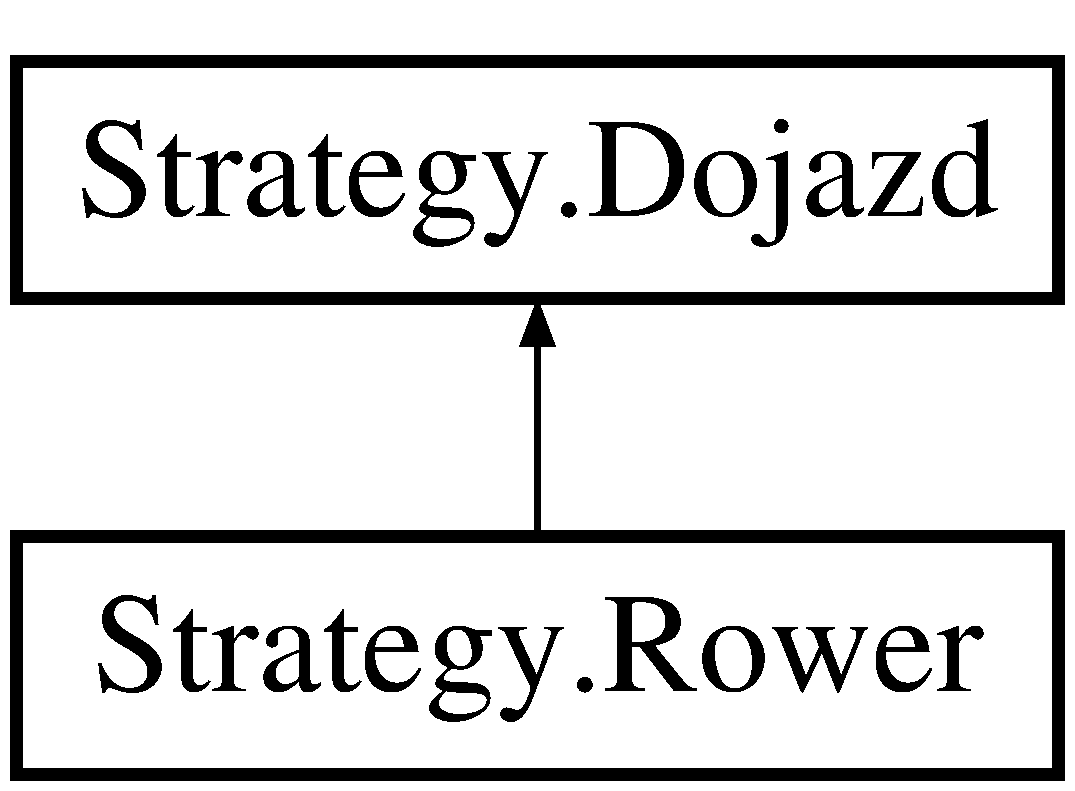
\includegraphics[height=2.000000cm]{class_strategy_1_1_rower}
\end{center}
\end{figure}
\subsection*{Public Member Functions}
\begin{DoxyCompactItemize}
\item 
\mbox{\Hypertarget{class_strategy_1_1_rower_ad1ec4490ccb956129ded7726930c8636}\label{class_strategy_1_1_rower_ad1ec4490ccb956129ded7726930c8636}} 
void {\bfseries dojazd} ()
\end{DoxyCompactItemize}


\subsection{Detailed Description}
Klasa implementacji funkcje dojazd 



The documentation for this class was generated from the following file\+:\begin{DoxyCompactItemize}
\item 
Program.\+cs\end{DoxyCompactItemize}

\hypertarget{class_strategy_1_1_samochod}{}\section{Strategy.\+Samochod Class Reference}
\label{class_strategy_1_1_samochod}\index{Strategy.\+Samochod@{Strategy.\+Samochod}}


Klasa implementacji funkcje dojazd  


Inheritance diagram for Strategy.\+Samochod\+:\begin{figure}[H]
\begin{center}
\leavevmode
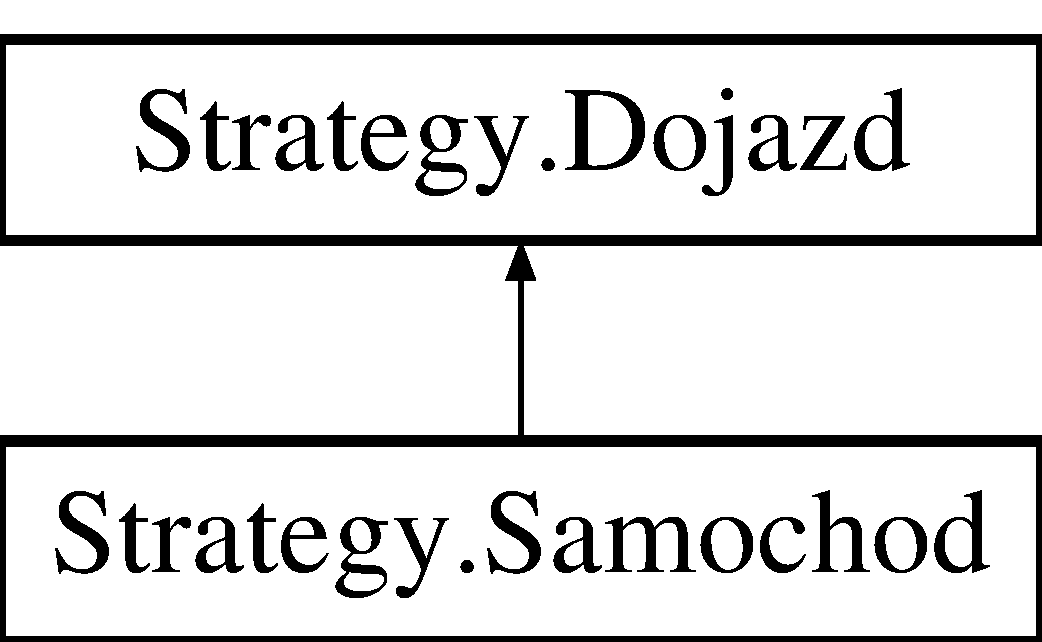
\includegraphics[height=2.000000cm]{class_strategy_1_1_samochod}
\end{center}
\end{figure}
\subsection*{Public Member Functions}
\begin{DoxyCompactItemize}
\item 
\mbox{\Hypertarget{class_strategy_1_1_samochod_a0e08ae22e6202ec3a0f6065f6885b048}\label{class_strategy_1_1_samochod_a0e08ae22e6202ec3a0f6065f6885b048}} 
void {\bfseries dojazd} ()
\end{DoxyCompactItemize}


\subsection{Detailed Description}
Klasa implementacji funkcje dojazd 



The documentation for this class was generated from the following file\+:\begin{DoxyCompactItemize}
\item 
Program.\+cs\end{DoxyCompactItemize}

\hypertarget{class_strategy_1_1_silownia}{}\section{Strategy.\+Silownia Class Reference}
\label{class_strategy_1_1_silownia}\index{Strategy.\+Silownia@{Strategy.\+Silownia}}


Klasa implementacji funkcje spedzaj\+Wolny\+Czas  


Inheritance diagram for Strategy.\+Silownia\+:\begin{figure}[H]
\begin{center}
\leavevmode
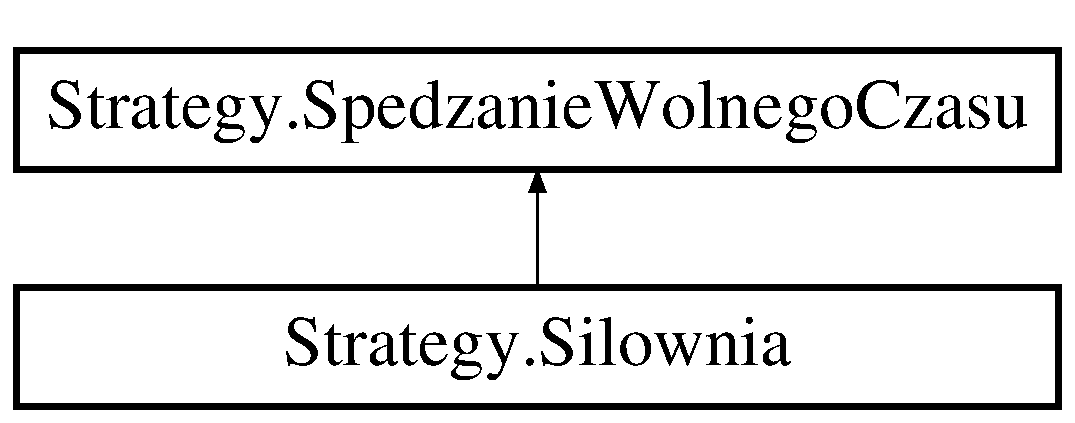
\includegraphics[height=2.000000cm]{class_strategy_1_1_silownia}
\end{center}
\end{figure}
\subsection*{Public Member Functions}
\begin{DoxyCompactItemize}
\item 
\mbox{\Hypertarget{class_strategy_1_1_silownia_a273e6ffeea532dcb14e8f40874443235}\label{class_strategy_1_1_silownia_a273e6ffeea532dcb14e8f40874443235}} 
void {\bfseries spedzaj\+Wolny\+Czas} ()
\end{DoxyCompactItemize}


\subsection{Detailed Description}
Klasa implementacji funkcje spedzaj\+Wolny\+Czas 



The documentation for this class was generated from the following file\+:\begin{DoxyCompactItemize}
\item 
Program.\+cs\end{DoxyCompactItemize}

\hypertarget{interface_strategy_1_1_spedzanie_wolnego_czasu}{}\section{Strategy.\+Spedzanie\+Wolnego\+Czasu Interface Reference}
\label{interface_strategy_1_1_spedzanie_wolnego_czasu}\index{Strategy.\+Spedzanie\+Wolnego\+Czasu@{Strategy.\+Spedzanie\+Wolnego\+Czasu}}


Interface wymagający implementacji funkcji spedzaj\+Wolny\+Czas  


Inheritance diagram for Strategy.\+Spedzanie\+Wolnego\+Czasu\+:\begin{figure}[H]
\begin{center}
\leavevmode
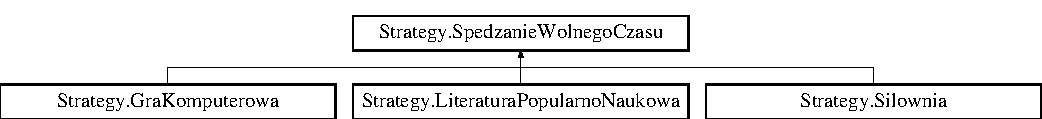
\includegraphics[height=1.588652cm]{interface_strategy_1_1_spedzanie_wolnego_czasu}
\end{center}
\end{figure}
\subsection*{Public Member Functions}
\begin{DoxyCompactItemize}
\item 
\mbox{\Hypertarget{interface_strategy_1_1_spedzanie_wolnego_czasu_a6b3d9e8040830b0a624da862dfe1d9c2}\label{interface_strategy_1_1_spedzanie_wolnego_czasu_a6b3d9e8040830b0a624da862dfe1d9c2}} 
void {\bfseries spedzaj\+Wolny\+Czas} ()
\end{DoxyCompactItemize}


\subsection{Detailed Description}
Interface wymagający implementacji funkcji spedzaj\+Wolny\+Czas 



The documentation for this interface was generated from the following file\+:\begin{DoxyCompactItemize}
\item 
Program.\+cs\end{DoxyCompactItemize}

\hypertarget{class_strategy_1_1_strategy}{}\section{Strategy.\+Strategy Class Reference}
\label{class_strategy_1_1_strategy}\index{Strategy.\+Strategy@{Strategy.\+Strategy}}


Klasa posiadająca funkcje Main  


\subsection*{Static Public Member Functions}
\begin{DoxyCompactItemize}
\item 
\mbox{\Hypertarget{class_strategy_1_1_strategy_a2fc010052482408caae24ab2a267d3c5}\label{class_strategy_1_1_strategy_a2fc010052482408caae24ab2a267d3c5}} 
static void {\bfseries Main} (string\mbox{[}$\,$\mbox{]} args)
\end{DoxyCompactItemize}


\subsection{Detailed Description}
Klasa posiadająca funkcje Main 



The documentation for this class was generated from the following file\+:\begin{DoxyCompactItemize}
\item 
Program.\+cs\end{DoxyCompactItemize}

\hypertarget{class_strategy_1_1_testuje_samochodow}{}\section{Strategy.\+Testuje\+Samochodow Class Reference}
\label{class_strategy_1_1_testuje_samochodow}\index{Strategy.\+Testuje\+Samochodow@{Strategy.\+Testuje\+Samochodow}}


Klasa implementacji funkcje pracuj  


Inheritance diagram for Strategy.\+Testuje\+Samochodow\+:\begin{figure}[H]
\begin{center}
\leavevmode
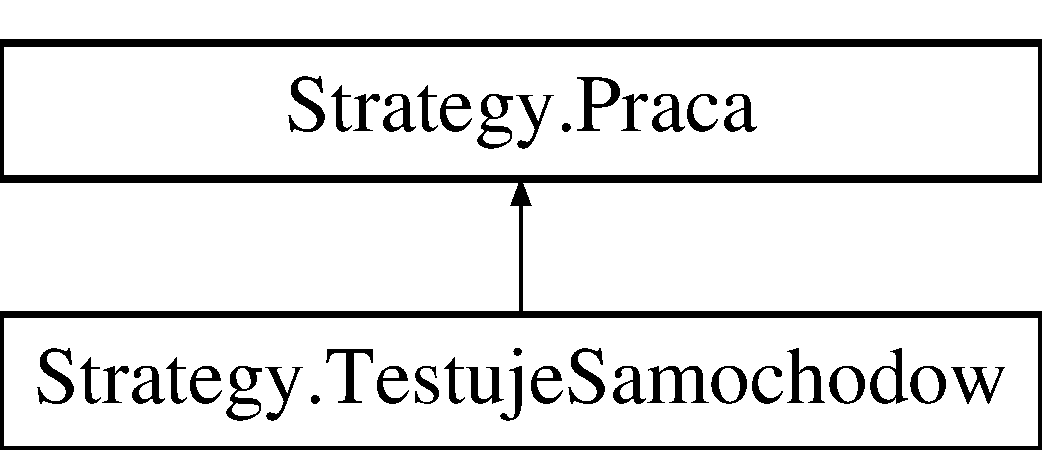
\includegraphics[height=2.000000cm]{class_strategy_1_1_testuje_samochodow}
\end{center}
\end{figure}
\subsection*{Public Member Functions}
\begin{DoxyCompactItemize}
\item 
\mbox{\Hypertarget{class_strategy_1_1_testuje_samochodow_a1ebd8f6a3af21e92198e871cc1610f16}\label{class_strategy_1_1_testuje_samochodow_a1ebd8f6a3af21e92198e871cc1610f16}} 
void {\bfseries pracuj} ()
\end{DoxyCompactItemize}


\subsection{Detailed Description}
Klasa implementacji funkcje pracuj 



The documentation for this class was generated from the following file\+:\begin{DoxyCompactItemize}
\item 
Program.\+cs\end{DoxyCompactItemize}

%--- End generated contents ---

% Index
\backmatter
\newpage
\phantomsection
\clearemptydoublepage
\addcontentsline{toc}{chapter}{Index}
\printindex

\end{document}
